\section{Joint inversion}\label{sec:joint}
The term joint inversion denotes the simultaneous inversion of a number of different data types.
We can classify different types according to the relation of the associated parameters:
\begin{enumerate}
	\item Identical parameters is historical the classical joint inversion, e.g. both DC and EM aim at $\rho$.
	\item Parameters are indirectly connected by petrophysical relations, e.g. ERT and GPR both aiming at water content.
	\item The parameters are independent. In this case only the structures can be linked to each other. For simple models this can involve the inversion of the geometry. For fixed models structural information is exchanged\footnote{Note that this type is formally a structurally coupled cooperative inversion.}.
\end{enumerate}

%%%%%%%%%%%%%%%%%%%%%%%%%%%%%%%%%%%%%%%%%%%%%%%%%%%%%%%%%%%%%%%%%%%%%%%%%%%
\subsection{Classical joint inversion of DC and EM soundings}\label{sec:jointdcem}
File \file{doc/tutorial/code/joint/dc\_mt\_joint1d.cpp}\\
First, let us consider to jointly invert different electromagnetic methods, e.g. direct current and MT\footnote{Of course AMT is usually done differently, however the use of MT data shows how it works.} data.
Both previously used methods are based on the same model (block model or smooth model) and yield an apparent resistivity vector.
In the common response function the two vectors are combined.
We create a new modelling class that derives from the DC1d modelling class\footnote{In order to use the classes, dc1dmodelling.h and em1dmodelling.h have to be included.} and has a member of the MT1d modelling class type.

\begin{lstlisting}[language=C++,morekeywords={RVector,RMatrix}]
class DC_MT_Modelling : public DC1dModelling {
public:
    DCMTModelling(Mesh & mesh,DataContainer & data,RVector & T,size_t nlay)
    : DC1dModelling( mesh, data, nlay, verbose ) { 
            fMT_ = new MT1dModelling( mesh, T, nlay, verbose );
    }
    virtual ~DC_MT_Modelling(){ delete fMT_; } //~fMT_(); }
    RVector response( const RVector & model ){
       return cat( DC1dModelling::response( model ), fMT_->rhoa( model ) );
    }
protected:
    MT1dModelling *fMT_;
};
\end{lstlisting}

The constructor initializes the parent class and the member class as used before.
In the response function both response functions are called and combined using the cat command.
That's it! The inversion is initialized with the combined apparent resistivities and runs as usual.

%%%%%%%%%%%%%%%%%%%%%%%%%%%%%%%%%%%%%%%%%%%%%%%%%%%%%%%%%%%%%%%%%%%%%%%%%%%
\subsection{Block joint inversion of DC/MRS data}\label{sec:blockjoint}
%File \file{doc/tutorial/code/joint/dc\_mt\_block1d.cpp}\\
If the underlying parameters of the jointed inversion are independent, a combination can only be achieved via the geometry.
For the case of a block 1d discretization both methods are affected by the layer thicknesses.
%We use the same methods as before \sperre

Similar to the above example, we create a combined modelling class that is derived from one method, in this case \lstinline|MRS1DBlockModelling|.
This one is a block model (water content and thickness) variant of the magnetic resonance sounding (MRS) modelling \lstinline|MRSModelling|.
The class has a DC resistivity forward modelling and holds the number of layers \lstinline|nlay|.

The model is created in the constructor using \lstinline|createMesh1DBlock( nlay, 2 )| that is able to hold, additionally to the thickness (region 0), multiple properties, here water content (region 1) and resistivity (region 2).
From the model vector the thickness, water content (or their combination) and resistivity has to be extracted and the result of the two forward calls are combined using the cat command.
The Jacobian is by default brute force, which is quite cheap for block models.

\begin{lstlisting}[language=C++,morekeywords={RVector,RMatrix}]
class DC_MRS_BlockModelling : public MRS1dBlockModelling{
public:
    DC_MRS_BlockModelling( size_t nlay, DataContainer & data, RMatrix & KR,
                           RMatrix & KI, RVector & zvec, bool verbose ) :
        MRS1dBlockModelling( nlay, KR, KI, zvec, verbose ), nl_( nlay ) { 
            setMesh( createMesh1DBlock( nlay, 2 ) ); //two-properties
            Mesh mymesh = createMesh1DBlock( nlay ); //single block mesh
            fDC_ = new DC1dModelling( mymesh, data, nlay, verbose );
        }
    virtual ~DC_MRS_BlockModelling( ){ delete fDC_; }
    
    RVector response( const RVector & model ){
        //! extract resistivity, watercontent & thickness from model vec
        RVector thk( model, 0 , nl_ - 1 );
        RVector wcthk( model, 0 , nl_ * 2 - 1 );
        RVector res( model, nl_ * 2 - 1 , nl_ * 3 - 1 );
        return cat( MRS1dBlockModelling::response( wcthk ), 
                    fDC_->rhoa( res, thk ) );
    }
protected:
    DC1dModelling *fDC_;
    int nl_;
};
\end{lstlisting}

In order to use the class, we have to build a cumulative data transform as in subsection \ref{sec:mt1d}.
Model transformations are logarithmic to ensure positive values, additionally an upper bound of 0.4 is defined for the water content.
\begin{lstlisting}[language=C++,morekeywords={RVector,RMatrix}]
    RTrans transVolt;    // linear voltages
    RTransLog transRhoa; // logarithmic apparent resistivities
    CumulativeTrans< RVector > transData;
    transData.push_back( transVolt, errorMRS.size() );
    transData.push_back( transRhoa, dataDC.size() );
    RTransLog transRes;
    RTransLogLU transWC(0.0, 0.4);
    RTransLog transThk;
\end{lstlisting}

In order to achieve a Marquardt inversion scheme, the constraint type is set to zero for all regions:
\begin{lstlisting}
    f.regionManager().setConstraintType( 0 );
\end{lstlisting}
Appropriately, the transformations and starting values are set.
\begin{lstlisting}
    f.region( 0 )->setTransModel( transThk );
    f.region( 0 )->setStartValue( 5.1 );
    f.region( 1 )->setTransModel( transWC );
    f.region( 1 )->setStartValue( 0.1 );
    f.region( 2 )->setTransModel( transRes );
    f.region( 2 )->setStartValue( median( dataDC.rhoa() ) );
\end{lstlisting}

We use a synthetic model of three layers representing a vadoze zone ($\rho=500\Omega$m, 0.1\% water, 4m thick), a saturated zone ($\rho=100\Omega$m, 40\% water content, 10m thick) and a bedrock ($\rho=2000\Omega$m, no water).
3\,\% and 20\,nV Gaussian noise are added to the DC and MRS data, respectively.
Figure~\ref{fig:blockjoint} shows the result of the combined inversion, which is very close to the synthetic model due to the improved information content from two models.

\begin{figure}[htb]
\centering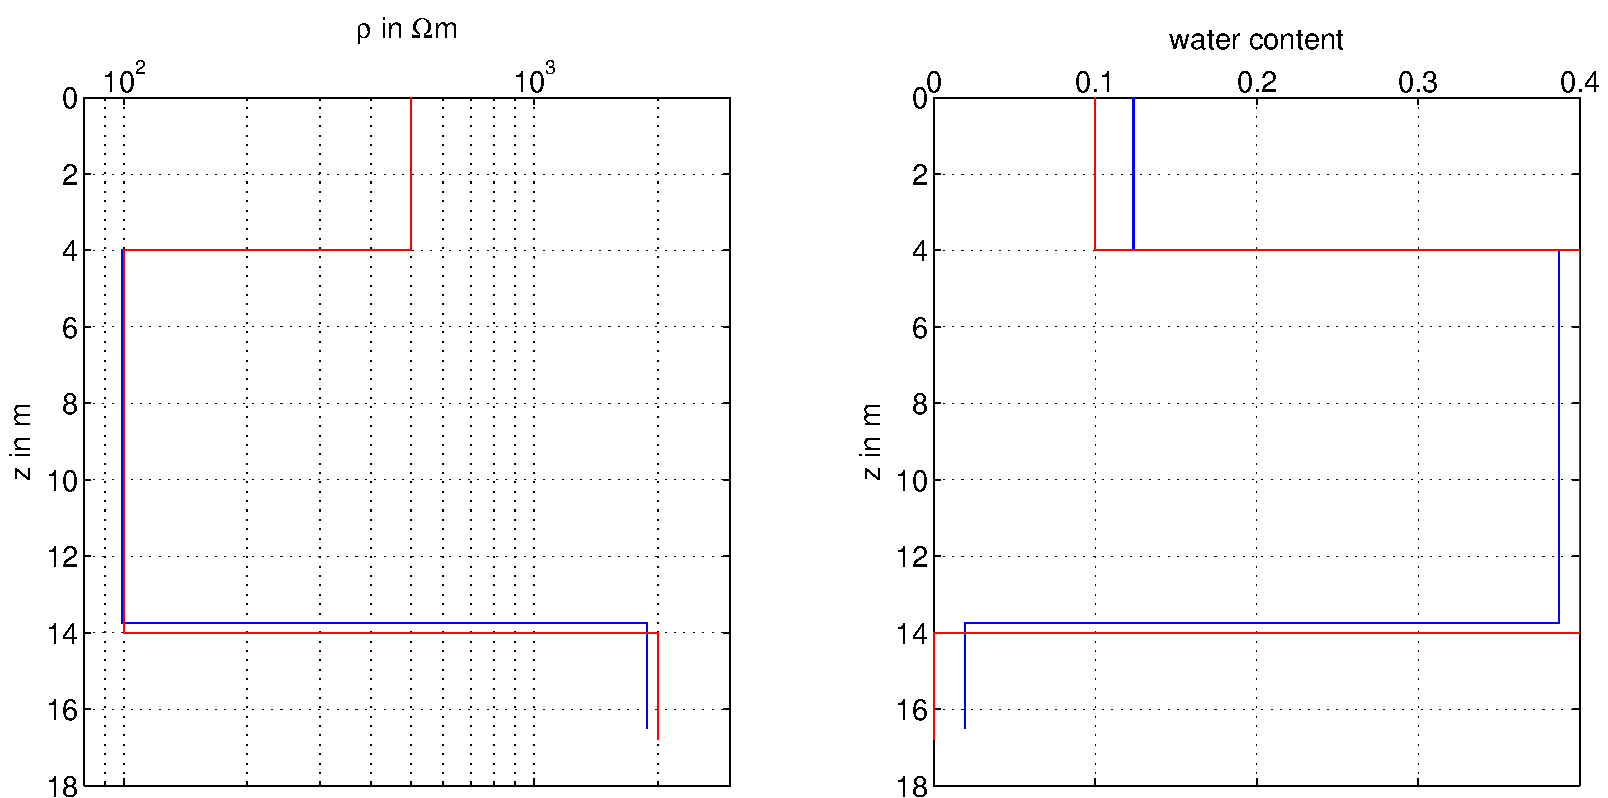
\includegraphics[width=0.9\textwidth]{dc_mrs_blockjoint}
\caption{Joint inversion result of block-coupled DC resistivity (left) and MRS (right) sounding.}\label{fig:blockjoint}
\end{figure}


%%%%%%%%%%%%%%%%%%%%%%%%%%%%%%%%%%%%%%%%%%%%%%%%%%%%%%%%%%%%%%%%%%%%%%%%%%%
\subsection{Structurally coupled cooperative inversion of DC and MRS soundings}\label{sec:structjoint}
File \file{doc/tutorial/code/joint/dc\_mrs\_joint1d.cpp}\\
In many cases it is not clear whether the model boundaries observed by different methods are identical or how many of them are existing.
Nevertheless we expect a similarity of the structure, i.e. the gradients.
On smooth model discretizations of any dimension the exchange of geometrical information can be achieved using the constraint control function \citep{guerue06nearsurface}.
Main idea is to decrease the weight for the roughness operator of one method depending on the partial derivative of the other.
A large roughness as a possible interface should enable the interface on the other side by a low weight.
There are different possible functions for doing so.
Originally, a iteratively reweighted least squares scheme was proposed that incorporates the whole distribution.
Here we use a simple function
\begin{equation}
    w_c(r) = \frac{a}{|r|+a}+a
\end{equation}
where $w_c$ is the weight, $r$ is the roughness value and $a$ is a small quantity.
For $r\rightarrow 0$ the weight $w_c=1+a$ lies slightly above 1, for $r\rightarrow\infty$ it becomes $a$.

In this case we apply it to DC resistivity and MRS sounding for a smooth 1d model.
The latter operator is linear and thus realized by a simple matrix vector multiplication of the kernel function and the water content vector.
We initialise the two independent inversions and run one iteration step each.
In the iteration loop we calculate the function of one roughness and set it as constraint weight for the other before running another inversion step.
\begin{lstlisting}
    invMRS.setMaxIter( 1 );
    invDC.setMaxIter( 1 );
    invMRS.run(); //! init and run 1 step
    invDC.run(); //! init and run 1 step
    double a = 0.1;
    RVector cWeight( nlay - 1 );
    for ( int iter = 1; iter < maxIter; iter++ ) {
        cWeight = a / ( abs( invDC.roughness() ) + a ) + a;
        invMRS.setCWeight( cWeight );
        cWeight = a / ( abs( invMRS.roughness() ) + a ) + a;
        invDC.setCWeight( cWeight );
        invDC.oneStep();
        invMRS.oneStep();
    }
\end{lstlisting}

Figure \ref{fig:dcmrsstruct} shows the inversion result for the above mentioned three-layer case.
Without coupling (a) the transitions between the layers are quite smooth.
Much more significant jumps in both parameters occur when structural coupling is applied (b) and make the interpretation of both layer thickness and representative parameters less ambiguous.

\begin{figure}[htb]
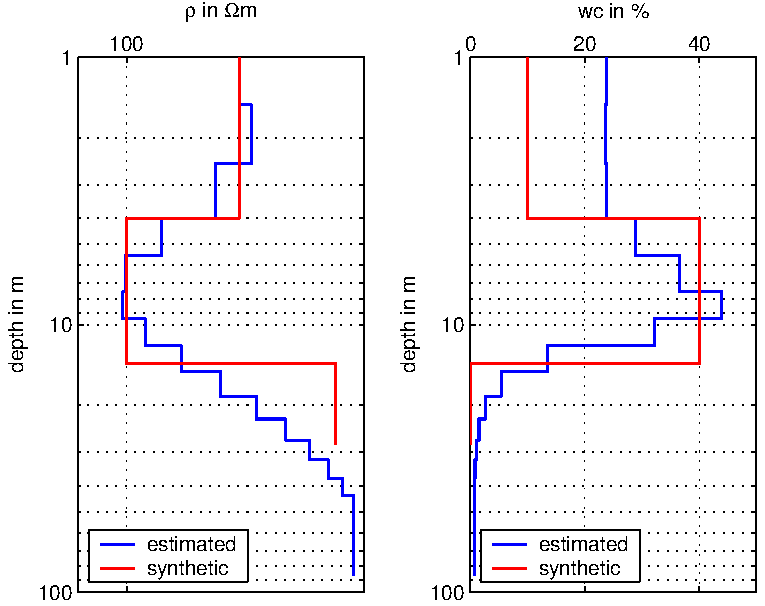
\includegraphics[width=0.5\textwidth]{DC-MRS-uncoupled}
\hfill
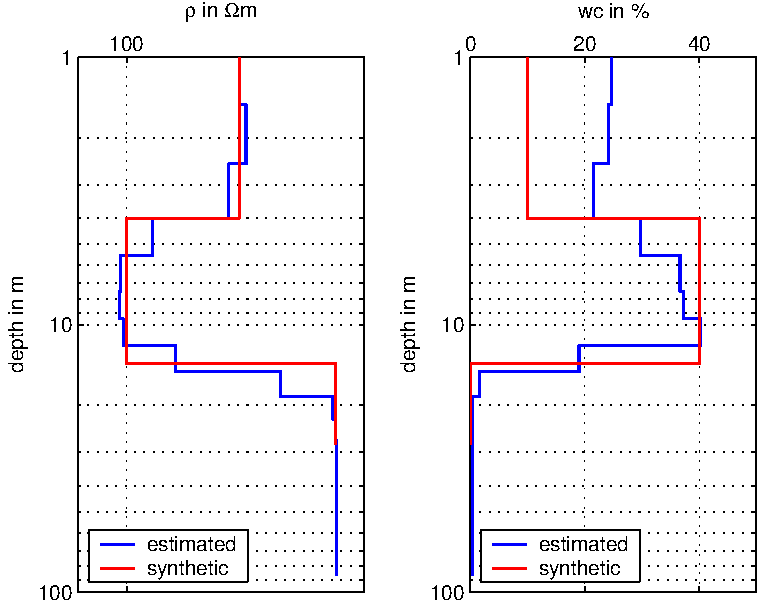
\includegraphics[width=0.5\textwidth]{DC-MRS-coupled}\\
\vskip -2ex 
a\hfill b%\\[1ex]
\caption{Synthetic model (red) and inversion results (blue) for DC (left) and MRS (right) 1D inversion without (a) and with (b) structural coupling}\label{fig:dcmrsstruct}
\end{figure} 

Of course the coupling does not have to affect the whole model.
The constraint weight vector can as well be set for an individual region such as the aquifer.
See inversion templates on how to do structural coupled inversion more easily and flexibly.

%%%%%%%%%%%%%%%%%%%%%%%%%%%%%%%%%%%%%%%%%%%%%%%%%%%%%%%%%%%%%%%%%%%%%%%%%%%
\subsection{Petrophysical joint inversion}\label{sec:petrojoint}
Target: water content in a soil column using GPR (CRIM equation) and DC (Archie equation)

\sperre{TO BE IMPLEMENTED}

\begin{figure}[htb]
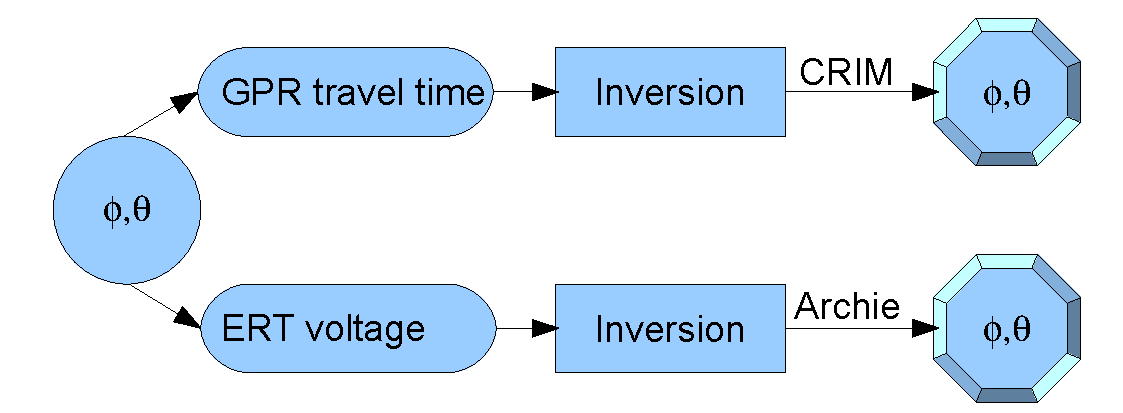
\includegraphics[width=0.5\textwidth]{petro1}
\hfill
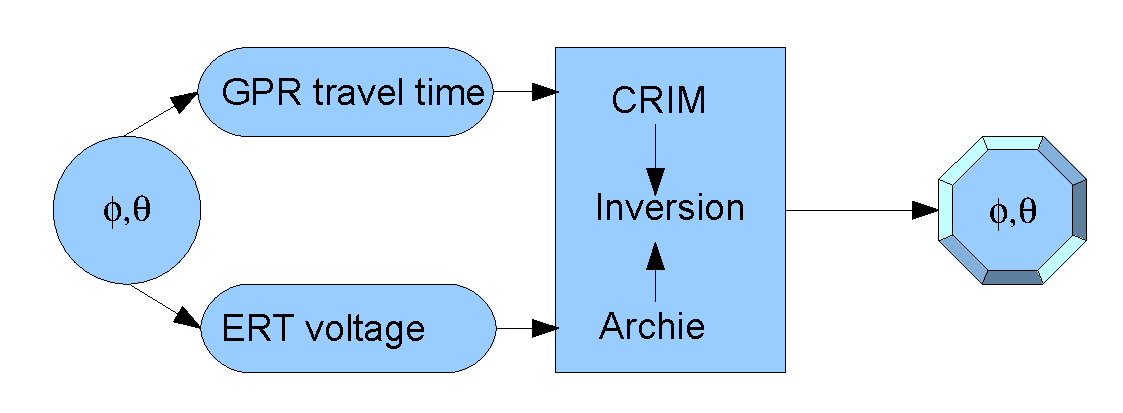
\includegraphics[width=0.5\textwidth]{petroji}\\
\vskip -8ex 
a\hfill b%\\[1ex]
\caption{Scheme for separate inversion (a) and petrophysical joint inversion (b) of GPR and ERT data to obtain an image of porosity or water content}\label{fig:petroji}
\end{figure} 
